
%----------------------------------------------------------------------------------------
%	Chapter 2
%----------------------------------------------------------------------------------------

\chapter{Basic Topology}

\bigbreak
\section{Finite, Countable, And Uncountable Sets}

\begin{defn}
	Consider two sets $A$ and $B$.
	If there exists a 1-1  mappmg of $A$ onto $B$, 
	we say that $A$ and $B$ can be put in 1-1 {\it correspondence}, 
	or that $A$ and B have the same {\it cardinal number}, 
	or, briefly, that $A$ and $B$ are {\it equivalent}, 
	and we write $A \sim B$. 
	
	This relation clearly has the following properties. 
	\begin{itemize}
		\item It is reflexive: $A \sim A$. 
		\item It is symmetric: If $A \sim B$, then $B \sim A$. 
		\item It is transitive: If $A \sim B$ and $B \sim C$, then $A \sim C$. 
	\end{itemize}
	Any relation with these three properties is  called an equivalence relation.
\end{defn}


\begin{defn}
	\label{count}
	For any integer $n$, let $J_n$ be the set whose elements are the integers $1, 2, \dots n$.
	Let $J$ be the set of all positive integers. For any set $A$, we say :
	\begin{enumerate}[(a)]
		\item $A$ is {\it finite} of $A \sim J_n$ for some $n$. (The empty set is also finite.)
		\item $A$ is {\it infinite} if it is not finite.
		\item $A$ is {\it countable} if $A \sim J$
		\item $A$ is {\it uncountable} if $A$ is neither finite nor countable.
		\item $A$ is {\it at most countable} if $A$ is finite or countable.
	\end{enumerate}
\end{defn}


\begin{exmp}
	Let $A$ be the set of all integers. Then $A$ is countable.
	Consider the following mapping :
	\begin{align*}
		A & : 0, 1, -1, 2, -2, 3, -3, \dots \\
		J & : 1, 2, 3, 4, 5, 6, 7, 8, \dots  
	\end{align*}
	We can even give an explicit formula for this :
	$$ 
	f(n) = 
	\begin{cases}
		\frac{n}{2} \quad (\text{n is even}) \\
		-\frac{(n-1)}{2} \quad (\text{n is odd})
	\end{cases}
	$$
\end{exmp}

\begin{rem}
	A finite set cannot be equivalent to one of its proper subsets. 
	This is, however, possible for infinite sets, is shown by the above example, 
	in which $J$ is a proper subset of $A$.

	In fact, we could replace definition \ref{count} by the statement: 
	$A$ is infinite if $A$ is equivalent to one of its proper subsets.
\end{rem}


\begin{defn}
	By a {\it sequence}, we mean a function $f$ defined on the set $J$ of all positive integers.
	If $f(n) = x_n$, for all $n \in J$. It is customary to denote the sequence $f$ by the symbol $\{ x_n \}$.
	If $A$ is a set and if $x_n \in A$ for all $n \in J$, then $\{x_n\}$ is said to be a {\it sequence} in $A$.
\end{defn}

\begin{thm}
	Every infinite subset of a countable set is countable.
	\begin{proof}
		Suppose $E \subseteq A$ and $E$ is infinite.
		Construct a sequence of distinct elements of $A$ and let it be $\{x_n\}$.
		Let $n_1$ be the smallest positive integer such that $x_{n_1} \in E$.
		Having chosen $n_1, n_2, \dots, n_{k-1}$, choose $n_k$ such that $n_k > n_{k-1}$
		and $x_{n_k} \in E$.

		Putting $f(k) = x_{n_k}$, we obtain a 1-1 correspondence between $E$ and $J$.

		The theorem roughly shows that countable sets represent the smallest infinity.
		No uncountable set can be subset of a countable set.
	\end{proof}
\end{thm}


\begin{thm}
	\label{count}
	Let $\{E_n\}, n = 1, 2, 3,\dots$ be a sequence of countable sets, and put
	$$ S = \bigcup_{n=1}^{\infty} E_n $$
	\begin{proof}
		Let every set $E_n$ be arranged in a sequence $\{x_{nk}\}, k = 1, 2, 3,\dots$, 
		and consider the infinite array,		
		\begin{figure}[ht!]
			\centering
			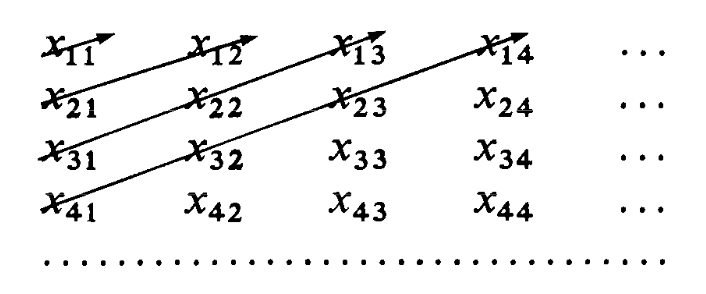
\includegraphics[scale=0.5]{./images/chapter_2_figure_1.png}
		\end{figure}
		in which the elements of $E_n$ form the $nth$ row.
		The array contains all elements of $S$. As indicated by the arrows, 
		these elements can be arranged in a sequence,
		$$ x_{11} ; x_{21}; x_{12}; x_{31}; \dots\dots\dots $$

		If any two of the sets $E_n$ have elements in common, 
		these will appear more than once. 
		Hence there is a subset $T$ of the set of all positive integers 
		such that $S \sim T$, which shows that $S$ is at most countable. 
		Since $E_1 \subset S$, and $E_1$ is infinite, $S$ is infinite, and thus countable.
	\end{proof}
\end{thm}

\begin{cor}
	Suppose $A$ is at most countable, and, for every $\alpha in A$, $B_{\alpha}$ is at most countable.
	Put $$ T = \bigcup_{\alpha \in A} B_{\alpha} $$
	Then $T$ is atmost countable.
\end{cor}

